% Condensate Partition Coefficient Pipeline — Instruction Manual
% Compile with pdfLaTeX (e.g. upload this folder to Overleaf and press Recompile).
% Figures are expected in ../figures (set via \graphicspath below).
\documentclass[11pt]{article}

\usepackage[margin=1in]{geometry}
\usepackage{graphicx}
\usepackage{booktabs}
\usepackage{array}
\usepackage{xcolor}
\usepackage{titlesec}
\usepackage{enumitem}
\usepackage{fancyhdr}
\usepackage{longtable}
\usepackage[T1]{fontenc}
\usepackage{lmodern}
\usepackage[colorlinks=true,linkcolor=accent,urlcolor=accent]{hyperref}

\definecolor{accent}{HTML}{1A73E8}
\definecolor{ink}{HTML}{222222}
\definecolor{muted}{HTML}{555555}

\graphicspath{{figures/}{../figures/}}

\titleformat{\section}{\Large\bfseries\color{accent}}{\thesection}{0.6em}{}
\titleformat{\subsection}{\large\bfseries\color{ink}}{\thesubsection}{0.6em}{}

\pagestyle{fancy}
\fancyhf{}
\lhead{\small\color{muted}Condensate Partition Coefficient Pipeline}
\rhead{\small\color{muted}Franco Lab · UCLA}
\cfoot{\small\color{muted}\thepage}
\renewcommand{\headrulewidth}{0.4pt}

\newcommand{\code}[1]{\texttt{\small #1}}

\begin{document}

% ─── Title page ───────────────────────────────────────────────────────────────
\begin{titlepage}
\centering
\vspace*{3cm}
{\color{accent}\Huge\bfseries Condensate Partition\\[0.3em] Coefficient Pipeline\par}
\vspace{1cm}
{\Large Instruction Manual\par}
\vspace{2cm}
{\large Automated 3D segmentation of nuclear biomolecular condensates\\
and measurement of the partition coefficient from confocal Z-stacks\par}
\vfill
{\large\bfseries Franco Lab \textbullet\ University of California, Los Angeles\par}
\vspace{0.4cm}
{\large Author: Daniel Chang\par}
{\large Principal Investigator: \rule{4cm}{0.4pt}\par} % ← fill in PI name
\vspace{0.8cm}
{\color{muted}Spring 2026\par}
\end{titlepage}

\tableofcontents
\newpage

% ─── Overview ─────────────────────────────────────────────────────────────────
\section{Overview}
This pipeline replaces the manual Imaris workflow for measuring the
\textbf{partition coefficient (PC)} of nuclear biomolecular condensates. Given a
two-channel confocal Z-stack, it segments nuclei and condensates in 3D, computes
the PC, and reports a calibrated value on the manual reference scale.

\begin{center}
\begin{tabular}{>{\raggedright}p{3.2cm} p{10cm}}
\toprule
\textbf{Inputs} & A two-channel Z-stack: channel 0 = nuclei, channel 1 = condensate.\\
\textbf{Outputs} & Nuclear \& cytoplasmic PC, 3D masks, per-object volumes, a summary figure.\\
\textbf{Validated on} & JABr: Pearson $r = 0.942$, MAE $12.9\%$, $79\%$ of cells within $\pm 20\%$ (n = 28).\\
\textbf{Interfaces} & Graphical (\code{run\_gui.py}) or command line (\code{pipeline.py}).\\
\bottomrule
\end{tabular}
\end{center}

\begin{center}
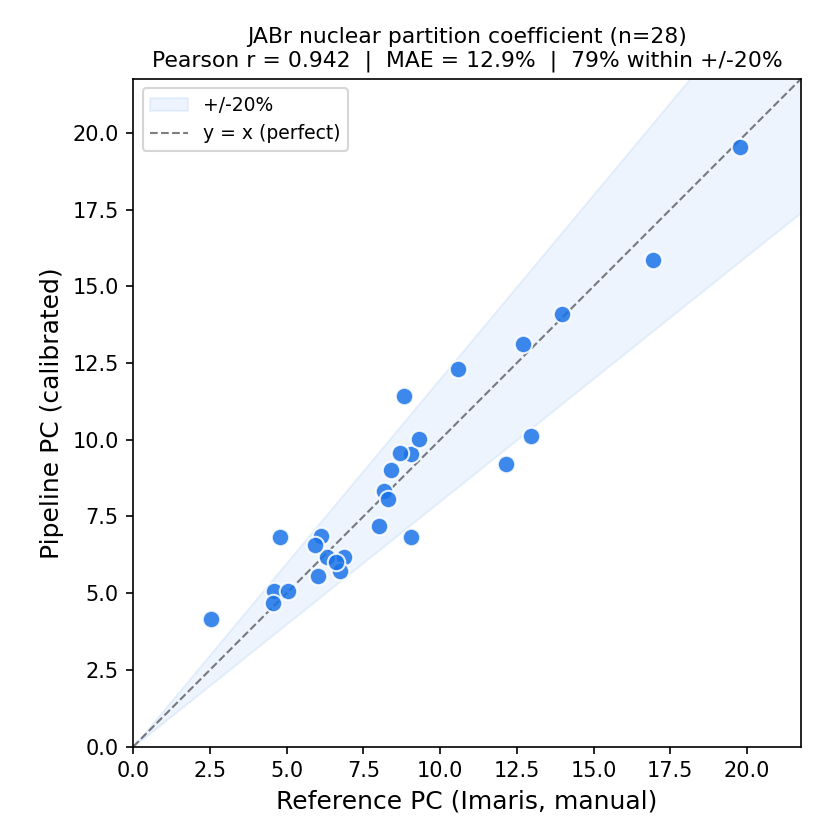
\includegraphics[width=0.62\textwidth]{jabr_validation.png}
\end{center}

% ─── Installation ─────────────────────────────────────────────────────────────
\section{Installation (one time)}
\begin{enumerate}[leftmargin=1.4em]
\item Install \textbf{Python 3.10 or 3.11}.
\item Install \textbf{PyTorch} for your machine from
\href{https://pytorch.org/get-started/locally/}{pytorch.org} (choose CPU or your
CUDA version). Example for CUDA 12.1:
\begin{quote}\code{pip install torch -{}-index-url https://download.pytorch.org/whl/cu121}\end{quote}
\item Install the remaining dependencies:
\begin{quote}\code{pip install -r requirements.txt}\end{quote}
\end{enumerate}
On first run, Cellpose downloads its model weights automatically (one-time
$\sim$100\,MB). A GPU is recommended ($\sim$10--15\,s per cell); CPU works but is
slower.

% ─── Input prep ───────────────────────────────────────────────────────────────
\section{Preparing your image files}
The pipeline accepts either one multi-channel TIF (both channels in one file) or
two separate single-channel TIFs. \textbf{Channel order matters:} channel 0 must
be nuclei, channel 1 the condensate. Most axis orderings (ZCYX, CZYX, \dots) are
auto-detected. If results look wrong, swapped channels are the most common cause.

% ─── GUI ──────────────────────────────────────────────────────────────────────
\section{Running with the graphical interface}
Launch with \code{python run\_gui.py}. A window with \textbf{Single File} and
\textbf{Batch} tabs opens.

\subsection{Step by step (single cell)}
\begin{enumerate}[leftmargin=1.4em]
\item On the \textbf{Single File} tab, choose the input mode (one multi-channel
TIF, or separate files) and \textbf{Browse\dots} to your data.
\item Choose an \textbf{Output} folder (optional).
\item In \textbf{Settings}, set \textbf{Construct = JABr}. For JABr, leave all
other settings at their defaults.
\item Click \textbf{\textcolor{accent}{$\blacktriangleright$ Run Pipeline}}. Progress
streams in the \textbf{Output Log}; the status reads \textbf{Done} when finished.
\item Open your output folder for the masks, tables, and \code{results.png}.
\end{enumerate}

\begin{quote}\color{muted}\small
\textit{Screenshots of the live GUI (\code{gui\_main.png}, \code{gui\_running.png},
\code{gui\_done.png}) should be captured on the machine where it runs
(Windows: \code{Win+Shift+S}) and placed in \code{docs/figures/}. The actual
numerical output of a real run is shown in Section~6.}
\end{quote}

% ─── Settings ─────────────────────────────────────────────────────────────────
\section{Understanding the settings}
For routine JABr analysis you only need to set \textbf{Construct}; the rest have
sensible defaults.

\renewcommand{\arraystretch}{1.25}
\begin{longtable}{>{\raggedright}p{3.4cm} >{\raggedright}p{1.6cm} p{8.5cm}}
\toprule
\textbf{Setting} & \textbf{Default} & \textbf{What it does}\\
\midrule
\endhead
Construct & (none) & Pick \textbf{JABr} for the validated workflow. Auto-selects the \code{blob\_log} detector \emph{and} the JABr calibration so the reported PC is on the manual scale.\\
Condensate detector & auto & \code{auto} routes JABr$\rightarrow$\code{blob\_log}, else Cellpose. Normally left on auto.\\
Top-X\% brightest voxels & 75 & Defines condensed-phase density; trims the dim mask halo to match the manual reference. Leave at 75.\\
Nuclei cell-prob.\ threshold & $-2.0$ & How aggressively nuclei are detected. $-2.0$ suits the lab's nuclear stain.\\
blob\_log threshold & 0.03 & Condensate spot-detection sensitivity (used when detector = \code{blob\_log}). Leave at 0.03 for JABr.\\
Cellpose cond.\ model path & (blank) & Advanced; a fine-tuned condensate model. Leave blank for JABr.\\
Disable GPU & off & Tick on a laptop with no NVIDIA GPU.\\
\bottomrule
\end{longtable}

\noindent\textbf{The one rule for routine use:} set \textbf{Construct = JABr} and
run. Everything else is for experimentation or other constructs.

% ─── Outputs ──────────────────────────────────────────────────────────────────
\section{Reading the outputs}
Every run writes: \code{summary.csv} (headline numbers incl.\ the calibrated PC),
\code{results.png} (summary figure), \code{condensate\_masks.tif} and
\code{nuclei\_masks.tif} (3D labeled masks), and per-object/per-slice CSVs.

For the bundled sample \code{JABr\_Sample2\_5\_3.tif}, a real run produces:
\begin{quote}\code{[nuclear] PC raw 4.867 $\rightarrow$ calibrated 4.813}\quad
(manual reference 4.558, $+5.6\%$)\end{quote}

\textbf{Report the calibrated nuclear PC} (the raw value is systematically
$\sim$3$\times$ the manual scale by construction; calibration standardizes it).
\textbf{Always glance at \code{condensate\_masks.tif}} over the raw channel in
Fiji/ImageJ --- a 10-second visual check catches the rare misfire.

\begin{center}
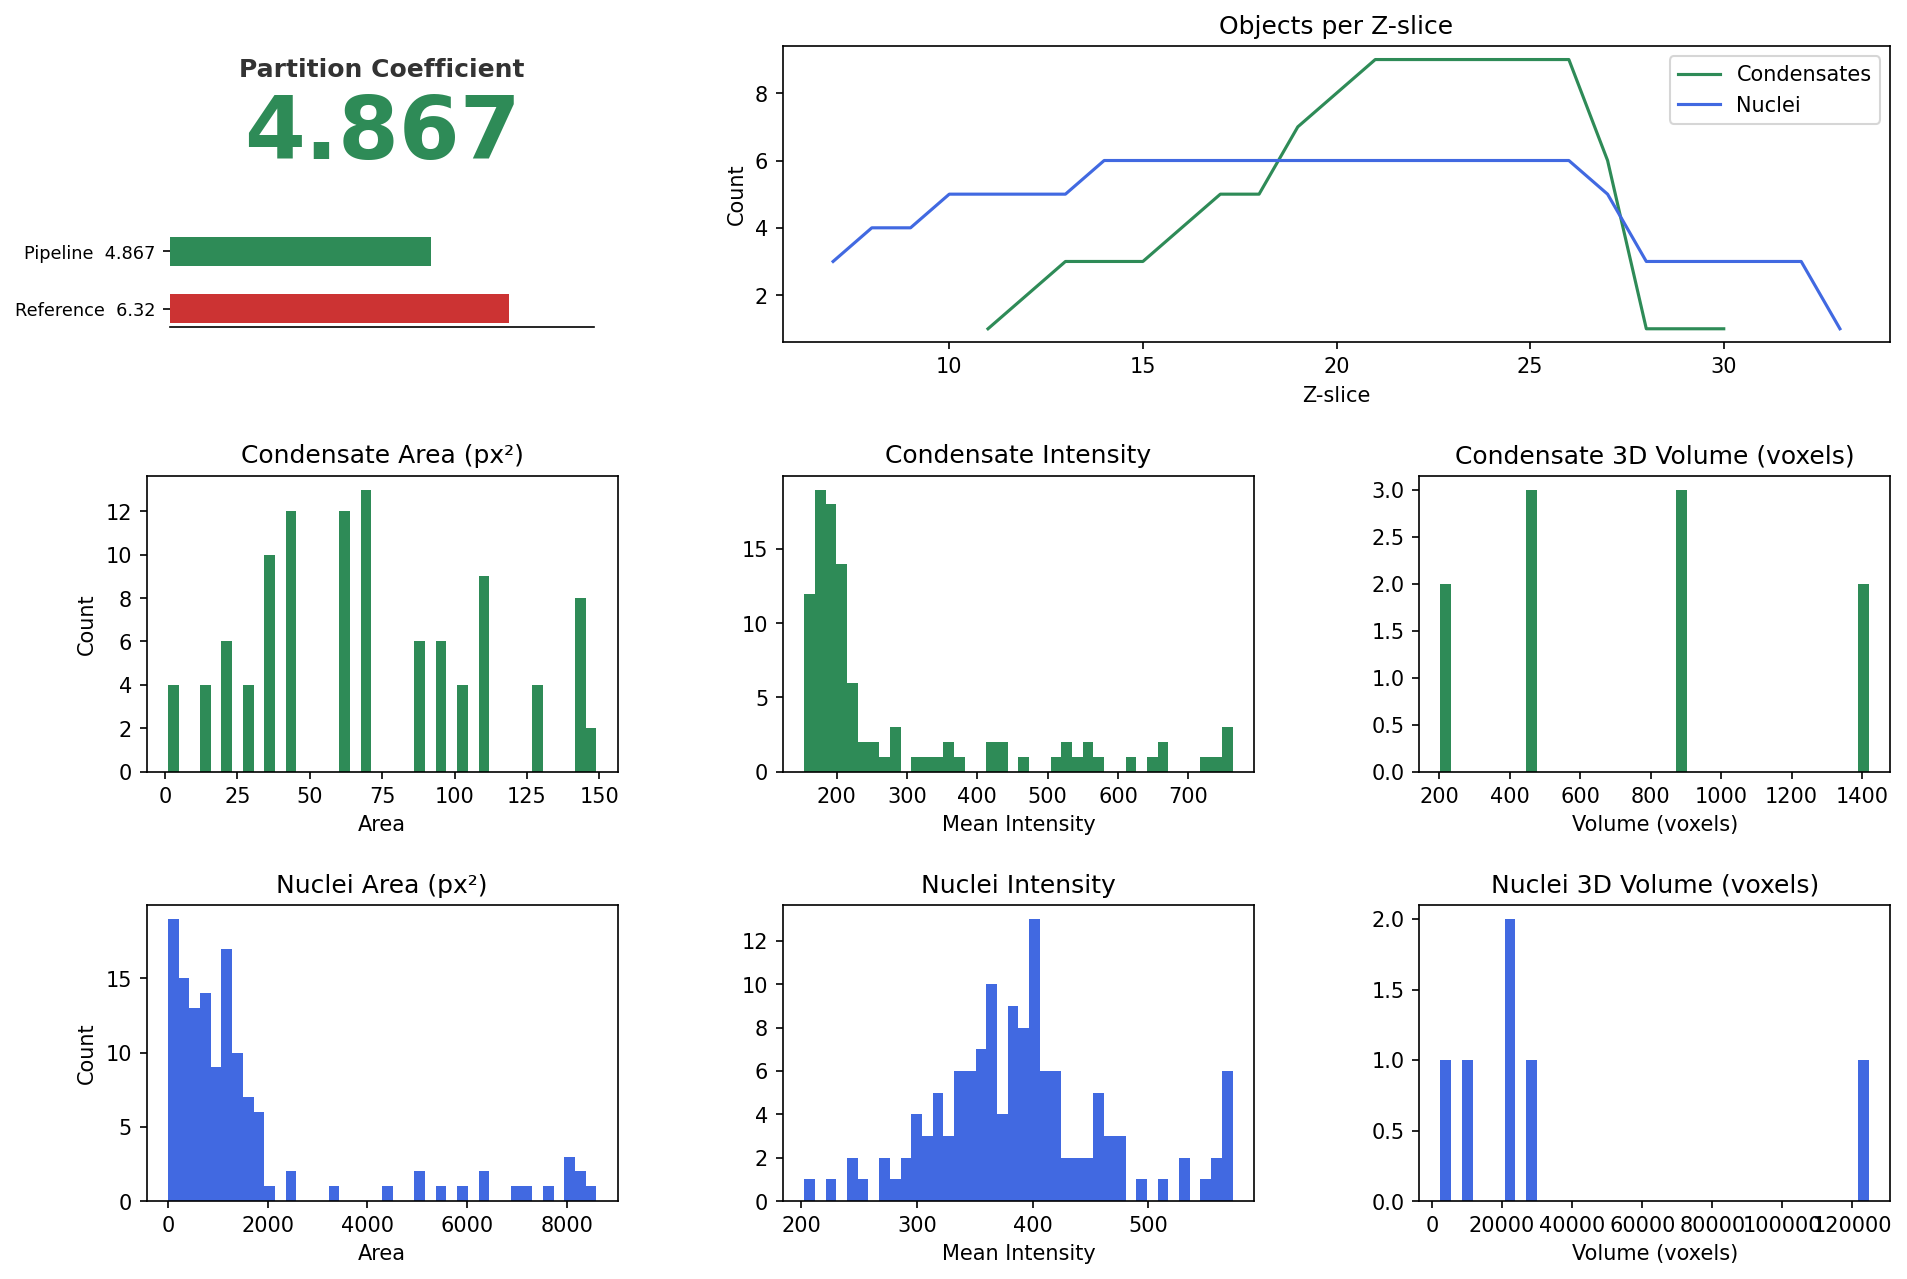
\includegraphics[width=0.95\textwidth]{example_results.png}\\
{\small\color{muted}\code{results.png} from the bundled-sample run.}
\end{center}

% ─── Batch ────────────────────────────────────────────────────────────────────
\section{Batch mode}
On the \textbf{Batch} tab, select a folder of \code{.tif} files; every file is
processed. Optionally supply the manual Imaris nuclear-PC CSV as a
\textbf{Reference CSV} --- the pipeline then writes \code{comparison.csv}
(pipeline vs manual, per cell) and \code{scatter.png} with the correlation, RMSE,
and MAE. Set \textbf{Construct = JABr} and run.

% ─── CLI ──────────────────────────────────────────────────────────────────────
\section{Command-line use}
\begin{quote}
\code{python pipeline.py -{}-roi sample\_data/JABr\_Sample2\_5\_3.tif -{}-construct JABr -{}-output my\_output}
\end{quote}
Separate channels: \code{-{}-nuc nuclei.tif -{}-cond condensate.tif}. Physical
volumes in $\mu m^3$: add \code{-{}-voxel-xy 0.065 -{}-voxel-z 0.3}. Force CPU:
\code{-{}-no-gpu}. For many files (and optional comparison against a manual
reference CSV), use the GUI \textbf{Batch} tab.

% ─── Troubleshooting ──────────────────────────────────────────────────────────
\section{Troubleshooting}
\begin{longtable}{>{\raggedright}p{5.5cm} p{8.0cm}}
\toprule
\textbf{Symptom} & \textbf{Likely cause / fix}\\
\midrule
\endhead
PC wildly off / nuclei look empty & Channels swapped: confirm ch0 = nuclei, ch1 = condensate.\\
``0 condensates detected'' & Not JABr, or very dim signal. Lower \code{blob\_log} threshold (e.g.\ 0.02); confirm the raw channel has spots.\\
Very slow (minutes per cell) & Running on CPU. Install a CUDA PyTorch build; ensure \textbf{Disable GPU} is unchecked.\\
\code{CUDA out of memory} & Tick \textbf{Disable GPU}, or close other GPU programs.\\
Cellpose download fails & First run needs internet for model weights.\\
One cell's calibrated PC looks off & Calibration is population-level; individual cells vary ($\pm 20\%$ for $\sim$80\% of cells). Verify against the mask.\\
\bottomrule
\end{longtable}

% ─── Method summary ───────────────────────────────────────────────────────────
\section{Method summary}
The PC is the ratio of condensed-phase to dilute-phase density (Fabrini et al.),
both camera-background-subtracted. Condensed density uses the brightest 75\% of
voxels inside (condensate $\cap$ nucleus); dilute density is the mean of the 50
lowest-intensity $10{\times}10{\times}10$ patches in the nuclear dilute region.
Nuclei are segmented with Cellpose 3 (\code{cyto3}, 3D), cleaned, and void-filled;
condensates are detected with Laplacian-of-Gaussian \code{blob\_log} and kept when
$\geq 50\%$ of the rendered sphere lies inside a nucleus. A per-construct linear
(JABr) or isotonic calibration standardizes the automated PC onto the manual
scale. Full rationale and the cross-construct scope/limits are in
\code{docs/METHODS.md}.

\vspace{1em}
\noindent\textbf{Scope.} Validated and production-ready for \textbf{JABr}. The
detector is construct-specific; a leave-one-construct-out test confirmed a single
detector does not generalize zero-shot (it under-detects on unseen constructs).
Extending to other constructs needs per-construct calibration or few-shot
retraining --- see \code{docs/METHODS.md}, Section 5.

\end{document}
